\documentclass{article}
\usepackage{tikz}
\usepackage{comment}
\usepackage[compat=1.0.0]{tikz-feynman}
\usetikzlibrary{shapes,arrows,positioning}
%=========================================================================
\tikzstyle{startstop} = [rectangle, rounded corners, minimum width=3cm, minimum height=1cm,text centered, draw=black, fill=red!30]
\tikzstyle{io} = [trapezium, trapezium left angle=70, trapezium right angle=110, minimum width=3cm, minimum height=1cm, text centered, draw=black, fill=blue!30]
\tikzstyle{process} = [rectangle,rounded corners, minimum width=3cm, minimum height=1cm, text centered, draw=black, fill=blue!30]
\tikzstyle{decision} = [diamond, minimum width=3cm, minimum height=1cm, text centered, draw=black, fill=green!30]
\tikzstyle{arrow} = [thick,->,>=stealth]
%==========================================================================
\begin{document}
	\title{Feynman diagrams : examples}
    \author{Raju}
	\maketitle
%============================================================================	
%	\section{Example 1}
%	\feynmandiagram [horizontal=a to b]{
%	i1--[fermion]a--[fermion]i2,
%	a--[photon]b,
%	f1--[fermion] b--[fermion] f2
%   };
	
	%========================================================================
%	\feynmandiagram [horizontal=a to b] {
%		i1 [particle=\(e^{-}\)] -- [fermion] a -- [fermion] i2 [particle=\(e^{+}\)],
%		a -- [photon, edge label=\(\gamma\), momentum'=\(k\)] b,
%		f1 [particle=\(\mu^{+}\)] -- [fermion] b -- [fermion] f2 [particle=\(\mu^{-}\)],
%	};
   %===========================================================================
   \section{example3}
	\begin{tikzpicture}
		\begin{feynman}
			\vertex (a) {\(\mu^{-}\)};
			\vertex [right=of a] (b);
			\vertex [above right=of b] (f1) {\(\nu_{\mu}\)};
			\vertex [below right=of b] (c);
			\vertex [above right=of c] (f2) {\(\overline \nu_{e}\)};
			\vertex [below right=of c] (f3) {\(e^{-}\)};
			
			\diagram* {
				(a) -- [fermion] (b) -- [fermion] (f1),
				(b) -- [boson, edge label'=\(W^{-}\)] (c),
				(c) -- [anti fermion] (f2),
				(c) -- [fermion] (f3),
			};
		\end{feynman}
	\end{tikzpicture}
%===================================================================
\section{QED}
 \begin{tikzpicture}
 	\begin{feynman}
 		\vertex(a) ;
 		\vertex [right=2cm of a] (b);
 		\vertex [above left=2cm of a](i1) {\( e^{-}\)};
 		\vertex [below left=2cm of a](i2) {\( e^{+}\)};
 		\vertex [above right=2cm of b](f1){\( \mu^{+} \)};
 		\vertex [below right=2cm of b](f2){\( \mu^{-} \)};
 		
 		\diagram*{
 			(i1)--[fermion](a)--[fermion](i2),
 			(a)--[photon, edge label'=\( \gamma \)](b),
 			(f1)--[fermion](b) ,
 			(b)--[fermion](f2) ,
 		};
 	\end{feynman}
 \end{tikzpicture}
%======================================================================
\section{QCD}
\hspace{3.5cm}
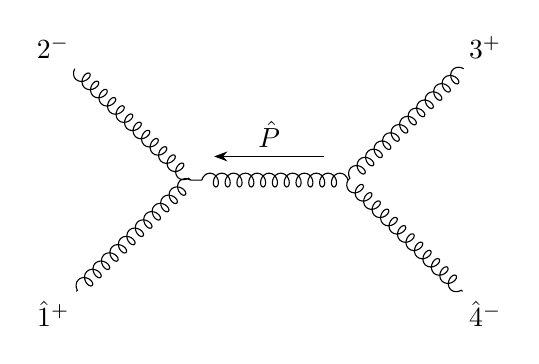
\begin{tikzpicture}
	\begin{feynman}
		\vertex(a) ;
		\vertex [right=2cm of a] (b);
		\vertex [above left=2cm of a](i1) {\( 2^{-} \)};
		\vertex [below left=2cm of a](i2) {\( \hat{1}^{+}\)};
		\vertex [above right=2cm of b](f1){\( 3^{+} \)};
		\vertex [below right=2cm of b](f2){\( \hat{4}^{-} \)};
		
		\diagram*{
			(i1)--[gluon](a)--[gluon](i2),
			(b)--[gluon, momentum'={[arrow style]\(\hat{P}\)}](a),
			(f1)--[gluon](b) ,
			(b)--[gluon](f2) ,
		};
	\end{feynman}
\end{tikzpicture}
\vspace{1cm}\\
%======================================================================
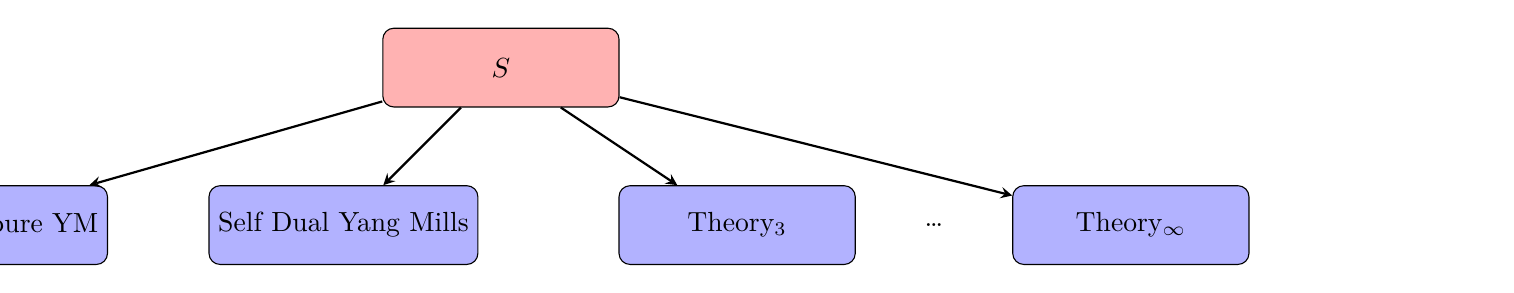
\begin{tikzpicture}[node distance=2cm]
	\hspace{-3cm}
	\node (start) [startstop] {$S$ };
	\node (ex1) [process, below of=start, xshift=-7cm] {MHV sector of pure YM}; 
	\node (ex2) [process, below of=start, xshift=-2cm] {Self Dual Yang Mills};
	\node (ex3) [process, below of=start, xshift=3cm] {Theory$_{3}$};
	\node (exn) [process, below of=start, xshift=8cm] {Theory$_{\infty}$};
	\draw [arrow] (start) -- (ex1);
	\draw [arrow] (start) -- (ex2);
	\draw [arrow] (start) -- (ex3);
	\draw [arrow] (start) -- (exn);
	%\draw[densely dotted](ex3)--node[]{}(exn);
	\path (ex3) -- node[auto=false]{\ldots} (exn);
\end{tikzpicture}
\vspace{1cm}\\
%=======================================================================
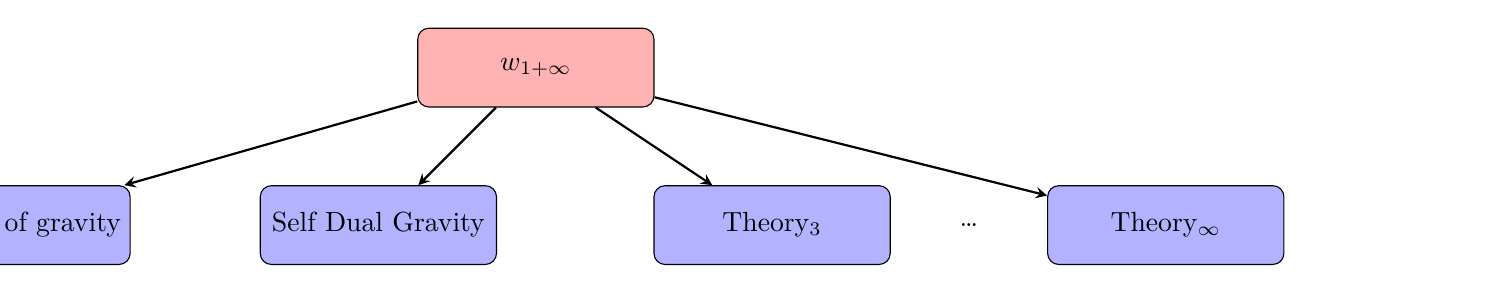
\begin{tikzpicture}[node distance=2cm]
	\hspace{-2.4cm}
	\node (start) [startstop] {$w_{1+\infty}$};
	\node (ex1) [process, below of=start, xshift=-7cm] {MHV sector of gravity}; 
	\node (ex2) [process, below of=start, xshift=-2cm] {Self Dual Gravity};
	\node (ex3) [process, below of=start, xshift=3cm] {Theory$_{3}$};
	\node (exn) [process, below of=start, xshift=8cm] {Theory$_{\infty}$};
	\draw [arrow] (start) -- (ex1);
	\draw [arrow] (start) -- (ex2);
	\draw [arrow] (start) -- (ex3);
	\draw [arrow] (start) -- (exn);
	%\draw[densely dotted](ex3)--node[]{}(exn);
	\path (ex3) -- node[auto=false]{\ldots} (exn);
\end{tikzpicture}
%======================================================================
\end{document}
